% Options for packages loaded elsewhere
\PassOptionsToPackage{unicode}{hyperref}
\PassOptionsToPackage{hyphens}{url}
%
\documentclass[
  ignorenonframetext,
]{beamer}
\usepackage{pgfpages}
\setbeamertemplate{caption}[numbered]
\setbeamertemplate{caption label separator}{: }
\setbeamercolor{caption name}{fg=normal text.fg}
\beamertemplatenavigationsymbolsempty
% Prevent slide breaks in the middle of a paragraph
\widowpenalties 1 10000
\raggedbottom
\setbeamertemplate{part page}{
  \centering
  \begin{beamercolorbox}[sep=16pt,center]{part title}
    \usebeamerfont{part title}\insertpart\par
  \end{beamercolorbox}
}
\setbeamertemplate{section page}{
  \centering
  \begin{beamercolorbox}[sep=12pt,center]{part title}
    \usebeamerfont{section title}\insertsection\par
  \end{beamercolorbox}
}
\setbeamertemplate{subsection page}{
  \centering
  \begin{beamercolorbox}[sep=8pt,center]{part title}
    \usebeamerfont{subsection title}\insertsubsection\par
  \end{beamercolorbox}
}
\AtBeginPart{
  \frame{\partpage}
}
\AtBeginSection{
  \ifbibliography
  \else
    \frame{\sectionpage}
  \fi
}
\AtBeginSubsection{
  \frame{\subsectionpage}
}
\usepackage{amsmath,amssymb}
\usepackage{iftex}
\ifPDFTeX
  \usepackage[T1]{fontenc}
  \usepackage[utf8]{inputenc}
  \usepackage{textcomp} % provide euro and other symbols
\else % if luatex or xetex
  \usepackage{unicode-math} % this also loads fontspec
  \defaultfontfeatures{Scale=MatchLowercase}
  \defaultfontfeatures[\rmfamily]{Ligatures=TeX,Scale=1}
\fi
\usepackage{lmodern}
\ifPDFTeX\else
  % xetex/luatex font selection
\fi
% Use upquote if available, for straight quotes in verbatim environments
\IfFileExists{upquote.sty}{\usepackage{upquote}}{}
\IfFileExists{microtype.sty}{% use microtype if available
  \usepackage[]{microtype}
  \UseMicrotypeSet[protrusion]{basicmath} % disable protrusion for tt fonts
}{}
\makeatletter
\@ifundefined{KOMAClassName}{% if non-KOMA class
  \IfFileExists{parskip.sty}{%
    \usepackage{parskip}
  }{% else
    \setlength{\parindent}{0pt}
    \setlength{\parskip}{6pt plus 2pt minus 1pt}}
}{% if KOMA class
  \KOMAoptions{parskip=half}}
\makeatother
\usepackage{xcolor}
\newif\ifbibliography
\usepackage{graphicx}
\makeatletter
\def\maxwidth{\ifdim\Gin@nat@width>\linewidth\linewidth\else\Gin@nat@width\fi}
\def\maxheight{\ifdim\Gin@nat@height>\textheight\textheight\else\Gin@nat@height\fi}
\makeatother
% Scale images if necessary, so that they will not overflow the page
% margins by default, and it is still possible to overwrite the defaults
% using explicit options in \includegraphics[width, height, ...]{}
\setkeys{Gin}{width=\maxwidth,height=\maxheight,keepaspectratio}
% Set default figure placement to htbp
\makeatletter
\def\fps@figure{htbp}
\makeatother
\setlength{\emergencystretch}{3em} % prevent overfull lines
\providecommand{\tightlist}{%
  \setlength{\itemsep}{0pt}\setlength{\parskip}{0pt}}
\setcounter{secnumdepth}{-\maxdimen} % remove section numbering
\ifLuaTeX
  \usepackage{selnolig}  % disable illegal ligatures
\fi
\IfFileExists{bookmark.sty}{\usepackage{bookmark}}{\usepackage{hyperref}}
\IfFileExists{xurl.sty}{\usepackage{xurl}}{} % add URL line breaks if available
\urlstyle{same}
\hypersetup{
  pdftitle={Introduction to Statistics},
  pdfauthor={John Karuitha},
  hidelinks,
  pdfcreator={LaTeX via pandoc}}

\title{Introduction to Statistics}
\author{John Karuitha}
\date{2023-09-18}

\begin{document}
\frame{\titlepage}

\begin{frame}{Introduction to Statistics}
\protect\hypertarget{introduction-to-statistics}{}
Background: In the mainstream media and social media, we are constantly
bombarded by a lot of data. In everyday language, the term data connotes
numerical types of data- population numbers, age, etc. However, much of
the data today is unstructured- from the music you listen to on Sportify
and YouTube Music, to videos you would watch on Netflix and YouTube. How
best can we make sense of this data? Statistics is the wing of maths
devoted to making sense of data? Note that not all data lends itself to
statistical analysis. In this course we examine how statistics allows us
to make sense of data. But first, some definitions.
\end{frame}

\begin{frame}{Defining statistics}
\protect\hypertarget{defining-statistics}{}
\begin{itemize}
\item
  The term statistics has several meanings;
\item
  Statistics the subject: Statistics is a way of reasoning, along with a
  collection of tools and methods, designed to help us understand the
  world.
\item
  Statistics as values computed: Statistics (plural) are quantities
  calculated from (sample) data.
\end{itemize}
\end{frame}

\begin{frame}{The two types of statistics - Descriptive vs Inferential}
\protect\hypertarget{the-two-types-of-statistics---descriptive-vs-inferential}{}
\begin{itemize}
\item
  Descriptive statistics is the term given to the analysis of data that
  helps describe, show or summarize data in a meaningful way such that,
  for example, patterns might emerge from the data.
\item
  Descriptive statistics do not, however, allow us to make conclusions
  beyond the data we have analysed or reach conclusions regarding any
  hypotheses we might have made.
\item
  They are simply a way to describe our data.
\item
  For instance, when you get a dataset with height and weight of
  students in your class and compute averages, variance and standard
  deviation.
\item
  HERE You are simply describing the data and NOT using it to make
  conclusions about the height and weight of ALL students at Karatina
  university.
\end{itemize}
\end{frame}

\begin{frame}{The two types of statistics - Descriptive vs Inferential}
\protect\hypertarget{the-two-types-of-statistics---descriptive-vs-inferential-1}{}
\begin{itemize}
\item
  In this level of statistics, we get data from a SAMPLE and use it to
  make conclusions about the WHOLE population.
\item
  Usually, we have no access to the entire population and rely on sample
  data to draw inferences about the population.
\item
  Example of inferential statistics is when you take a sample of 2nd
  year BPM students at Karatina University, take their height and
  weight, and use this data as a basis to infer the height and weight of
  ALL students at Karatina University.
\end{itemize}
\end{frame}

\begin{frame}{Defining data;}
\protect\hypertarget{defining-data}{}
\begin{itemize}
\item
  What are data? (singular- datum): Data are qualitative or quantitative
  values along with their context.
\item
  Modern datasets are so large; think of how much data safaricom
  collects in a day. Would you store that data in an excel spreadsheet.
  NO!
\item
  Usually large datasets are stored in vast repositories (databases)
  called data warehouses, and accessed by advanced tools like SQL. Find
  out what SQL is!!
\end{itemize}
\end{frame}

\begin{frame}{Big Data}
\protect\hypertarget{big-data}{}
\begin{itemize}
\item
  The sheer quantity of data has birthed a new name, big data.
\item
  Big data are data so vast they cannot be handled using the traditional
  methods of storage (e.g.~excel spreadsheet) and analysis (using SPSS)
  are inadequate.
\item
  Big data connotes data that accumulates very fast (the velocity
  problem), from many sources and in different varieties- text, video,
  pictures, sound (the variety problem), and is large in quantity (the
  volume problem) that it is challenging to tell whether or not it is
  authentic (the veracity problem- think of the modern prevalence of
  fake news on social media).
\item
  Think of a dataset with 150 billion rows of data and 1000 columns of
  variables. wheredo you start analysing that?
\end{itemize}
\end{frame}

\begin{frame}{Data Analytics;}
\protect\hypertarget{data-analytics}{}
\begin{itemize}
\item
  Many companies are increasingly using past customer data to predict
  their future purchases, which allows them to serve customers better or
  target them better with adverts.
\item
  This process of using data, especially of transactional data (data
  collected for recording the companies' transactions), to make
  decisions and predictions is sometimes called data mining or
  predictive analytics. The more general term business analytics (or
  sometimes simply analytics) describes any use of data and statistical
  analysis to drive business decisions from data whether the purpose is
  predictive or simply descriptive.
\end{itemize}
\end{frame}

\begin{frame}{Data context}
\protect\hypertarget{data-context}{}
To make sense of data we need to answer several questions;

\begin{itemize}
\item
  Who is the data about? Individuals, corporations, machines, etc.
\item
  What is the data is about? purchase history, weight, blood group, etc.
\item
  When was the data collected? is it still relevant if it was collected
  50 years ago?
\item
  Where were the data collected? Is data collected in Somalia relevant
  to Kenya.
\item
  Why was the data collected? What questions did we have in mind? For
  tax accounting purposes; For use in targeting adverts to consumers? In
  short what were your research questions?
\end{itemize}
\end{frame}

\begin{frame}{Metadata}
\protect\hypertarget{metadata}{}
\begin{itemize}
\item
  Metadata is data about data.
\item
  Check the last phone call you made.
\item
  The metadata about the call tells you who you called, when you called,
  the duration of the call including the data and time, if you ask
  safaricom they will give you data about where you called from,
  including a verbatim of what you discussed (the what and why you
  called).
\item
  Metadata allows us to aswer the who, what, when, where and why of
  data.
\item
  Metadata provides the context of the data.
\end{itemize}
\end{frame}

\begin{frame}{Storing data}
\protect\hypertarget{storing-data}{}
Usually data are stored in data tables.

\begin{itemize}
\item
  Most databases are just huge data tables.
\item
  Rows of the data table represent individual cases.
\item
  Columns of the data represent the variables- the attributes of each
  case.
\end{itemize}
\end{frame}

\begin{frame}[fragile]{Example of a data table}
\protect\hypertarget{example-of-a-data-table}{}
\begin{verbatim}
## 
## Attaching package: 'janitor'
\end{verbatim}

\begin{verbatim}
## The following objects are masked from 'package:stats':
## 
##     chisq.test, fisher.test
\end{verbatim}

\begin{verbatim}
## -- Attaching core tidyverse packages ------------------------ tidyverse 2.0.0 --
## v dplyr     1.1.3     v purrr     1.0.2
## v forcats   1.0.0     v readr     2.1.4
## v ggplot2   3.4.3     v stringr   1.5.0
## v lubridate 1.9.2     v tidyr     1.3.0
## -- Conflicts ------------------------------------------ tidyverse_conflicts() --
## x dplyr::filter()     masks stats::filter()
## x dplyr::group_rows() masks kableExtra::group_rows()
## x dplyr::lag()        masks stats::lag()
## i Use the conflicted package (<http://conflicted.r-lib.org/>) to force all conflicts to become errors
## 
## Attaching package: 'rvest'
## 
## 
## The following object is masked from 'package:readr':
## 
##     guess_encoding
\end{verbatim}

\begin{table}

\caption{\label{tab:unnamed-chunk-1}Data about men and women}
\centering
\begin{tabular}[t]{l|l|l|l|l|l}
\hline
Name & Age & Height & Weight & County & Date\_of\_data\\
\hline
Atieno & 32 & 180 & 90 & Mombasa & Jan 1, 2021\\
\hline
Mogaka & 25 & 160 & 70 & Laikipia & Jan 1, 2021\\
\hline
Etyang & 18 & 200 & 74 & Narok & Jan 1, 2021\\
\hline
Jeptoo & 22 & 150 & 55 & Wajir & Jan 1, 2021\\
\hline
Junior & 10 & 120 & 35 & Samburu & Jan 1, 2021\\
\hline
\end{tabular}
\end{table}
\end{frame}

\begin{frame}[fragile]{Data table}
\protect\hypertarget{data-table}{}
\begin{itemize}
\item
  Each row represents a case. For instance the first row tells us about
  Atieno, and so on.
\item
  Each row is a record, information about an individual in a database.
\item
  Cases go by different names, depending on the situation. Individuals
  who answer a survey are referred to as \texttt{respondents}. People on
  whom we experiment are \texttt{subjects} or (in an attempt to
  acknowledge the importance of their role in the experiment)
  \texttt{participants}, but animals, plants, websites, and other
  inanimate subjects are often called \texttt{experimental\ units}.
  Often we call cases just what they are: for example, customers,
  economic quarters, or companies. In a database, rows are called
  records---in this example, purchase records. Perhaps the most generic
  term is cases.
\end{itemize}
\end{frame}

\begin{frame}[fragile]{Data table}
\protect\hypertarget{data-table-1}{}
\begin{itemize}
\item
  The column titles (variable names) tell what has been recorded.
\item
  Each recorded item in the column is called a variable, like name,
  height, weight etc.
\item
  A general term for a data table like the one shown above is a
  \texttt{spreadsheet}, a name that comes from bookkeeping ledgers of
  financial information.
\item
  In large datasets many datatables are linked together in a
  \texttt{relational\ database} like we do in Ms Access.
\end{itemize}
\end{frame}

\begin{frame}{Variable Types}
\protect\hypertarget{variable-types}{}
\begin{itemize}
\item
  When the values of a variable are simply the names of categories we
  call it a categorical, or qualitative, variable. Examples are Name and
  County in our table.
\item
  When the values of a variable are measured numerical quantities with
  units, we call it a quantitative variable. Note they must have units
  to be quantitative.
\item
  BE CAREFUL;
\item
  Your National ID number is NOT quantitative!!!! Does it have units??
  If you were to get the mean of the ID Numbers of your family members,
  how would you interpret it?
\item
  Numbers like ID Numbers are identifier variables, just a special type
  of categorical or qualitative variables that you could easily confuse
  as quantitative.
\end{itemize}
\end{frame}

\begin{frame}{Identify qualitative vs categorical (qualitative)
variables}
\protect\hypertarget{identify-qualitative-vs-categorical-qualitative-variables}{}
\begin{itemize}
\item
  Admission number; 111, 112, 113, 114, 115
\item
  Height; Short, Medium, Tall, Tall, Short, Median
\item
  Height; 150 cm. 180 cm, 200 cm, 120 cm.
\item
  Weight: Underweight, Obese, Overweight, Ideal Weight, Overweight.
\item
  Weight: 60 kg, 170 kg, 90 kg, 75 kg
\item
  Age; Toddler, teen. teen, young adult, elder.
\item
  Age; 15 years, 20 years, 17 years.
\item
  Age; 15-20 years, 20-24 years, 50-60 years, 70 years and above.
\item
  Notice how variables can be presented as qualitative or quantitative
  (see height/ weight/age).
\end{itemize}
\end{frame}

\begin{frame}{Identify qualitative vs categorical (qualitative)
variables}
\protect\hypertarget{identify-qualitative-vs-categorical-qualitative-variables-1}{}
\begin{itemize}
\tightlist
\item
  Don't label a variable as categorical or quantitative without thinking
  about the data and what they represent. The same variable can
  sometimes take on different roles.
\item
  Don't assume that a variable is quantitative just because its values
  are numbers. Categories are often given numerical labels. Don't let
  that fool you into thinking they have quantitative meaning. Look at
  the context.
\item
  Always be skeptical. One reason to analyze data is to discover the
  truth. Even when you are told a context for the data, it may turn out
  that the truth is a bit (or even a lot) different. The context colors
  our interpretation of the data, so those who want to influence what
  you think may slant the context. A survey that seems to be about all
  students may in fact report just the opinions of those who visited a
  fan website. The question that respondents answered may be posed in a
  way that influences responses.
\end{itemize}
\end{frame}

\begin{frame}{Variables types}
\protect\hypertarget{variables-types}{}
\begin{itemize}
\item
  Categorical variables can either be ordinal vs nominal.
\item
  Weight; light, medium, heavy, superheavy
\item
  Age; Toddler, Teen, Young adult, Elder.
\item
  Note that these two categorical variables have inherent order; the are
  ordinal.
\item
  order == ordinal
\end{itemize}
\end{frame}

\begin{frame}{Variables types- Ordinal vs Nominal.}
\protect\hypertarget{variables-types--ordinal-vs-nominal.}{}
\begin{itemize}
\item
  Others have no inherent order, they are Nominal.
\item
  Examples are gender (male, female); names of cities (Nairobi, Mombasa,
  Kisumu)
\item
  Look at the county column in the table above, is there order; so are
  names.
\end{itemize}
\end{frame}

\begin{frame}{Variable types- continous or discrete}
\protect\hypertarget{variable-types--continous-or-discrete}{}
\begin{itemize}
\item
  Numeric variables are either continous or discrete.
\item
  Continous variables can take on any value inclusing fractions and
  zero.
\item
  Continuous variables are usually measured like height, weight, speed.
\item
  In many cases, variables like weight are usually shown as whole
  numbers but in reality can take on any values.
\item
  We mostly present continuous values as discrete because of convenience
  or lack of precise tools for measuring,
\item
  This problem of presenting continuous variables as discrete is called
  ``discretization''.
\item
  In reality, may be you are not 21 years old; you could be 21.01 years
  old if you put in the days, hours, minutes and seconds.
\end{itemize}
\end{frame}

\begin{frame}{Variable types- continous or discrete}
\protect\hypertarget{variable-types--continous-or-discrete-1}{}
\begin{itemize}
\item
  Other numeric variables are discrete- they can only take on whole
  numbers.
\item
  Can we have 2.5 students in a class?
\item
  Think of discrete numbers as counts.
\end{itemize}
\end{frame}

\begin{frame}{Data Types; Time series, cross-sectional, and logitudinal/
panel data}
\protect\hypertarget{data-types-time-series-cross-sectional-and-logitudinal-panel-data}{}
A time series is an ordered sequence of values of one or more
quantitative variables measured at regular intervals over time. Time
series are common in business. Typical measuring points are months,
quarters, or years, but virtually any consistently-spaced time interval
is possible.
\end{frame}

\begin{frame}{Example: Time series}
\protect\hypertarget{example-time-series}{}
\begin{table}

\caption{\label{tab:unnamed-chunk-2}An example of Time series data}
\centering
\begin{tabular}[t]{r|r|r}
\hline
Year & Salary & Weight\\
\hline
2010 & 10000 & 87.51761\\
\hline
2011 & 11000 & 81.98007\\
\hline
2012 & 12000 & 88.76610\\
\hline
2013 & 13000 & 81.59932\\
\hline
2014 & 14000 & 82.98576\\
\hline
2015 & 15000 & 83.05165\\
\hline
2016 & 16000 & 87.95527\\
\hline
2017 & 17000 & 80.56446\\
\hline
2018 & 18000 & 87.35103\\
\hline
2019 & 19000 & 88.15214\\
\hline
2020 & 20000 & 89.22783\\
\hline
\end{tabular}
\end{table}
\end{frame}

\begin{frame}{Cross sectional data}
\protect\hypertarget{cross-sectional-data}{}
\begin{itemize}
\item
  For cross-sectional data, several variables are measured at the same
  time point, see table 1.
\item
  The data in table 1 was all at a point in time, Jan 1, 2021.
\end{itemize}
\end{frame}

\begin{frame}{Panel data}
\protect\hypertarget{panel-data}{}
\begin{itemize}
\item
  Panel data has both a time series element and a cross-sectional
  element.
\item
  Research on this.
\end{itemize}
\end{frame}

\begin{frame}{Exercise}
\protect\hypertarget{exercise}{}
I dentify the data types in the following set of data.

\begin{table}

\caption{\label{tab:unnamed-chunk-3}World Population by Continent}
\centering
\fontsize{8}{10}\selectfont
\begin{tabular}[t]{rlrrrr}
\toprule
number & continent & population\_2023 & area\_km2 & density\_p\_km2 & world\_population\_share\\
\midrule
1 & Asia & 4753079726 & 31033131 & 153 & 59.08\\
2 & Africa & 1460481772 & 29648481 & 49 & 18.15\\
3 & Europe & 740433713 & 22134710 & 33 & 9.20\\
4 & North America & 604182517 & 21330000 & 28 & 7.51\\
5 & South America & 439719009 & 17461112 & 25 & 5.47\\
\addlinespace
6 & Australia/Oceania & 46004866 & 8486460 & 5 & 0.57\\
7 & Antarctica & 0 & 13720000 & 0 & 0.00\\
\bottomrule
\end{tabular}
\end{table}
\end{frame}

\begin{frame}{Exercise}
\protect\hypertarget{exercise-1}{}
\begin{figure}
\centering
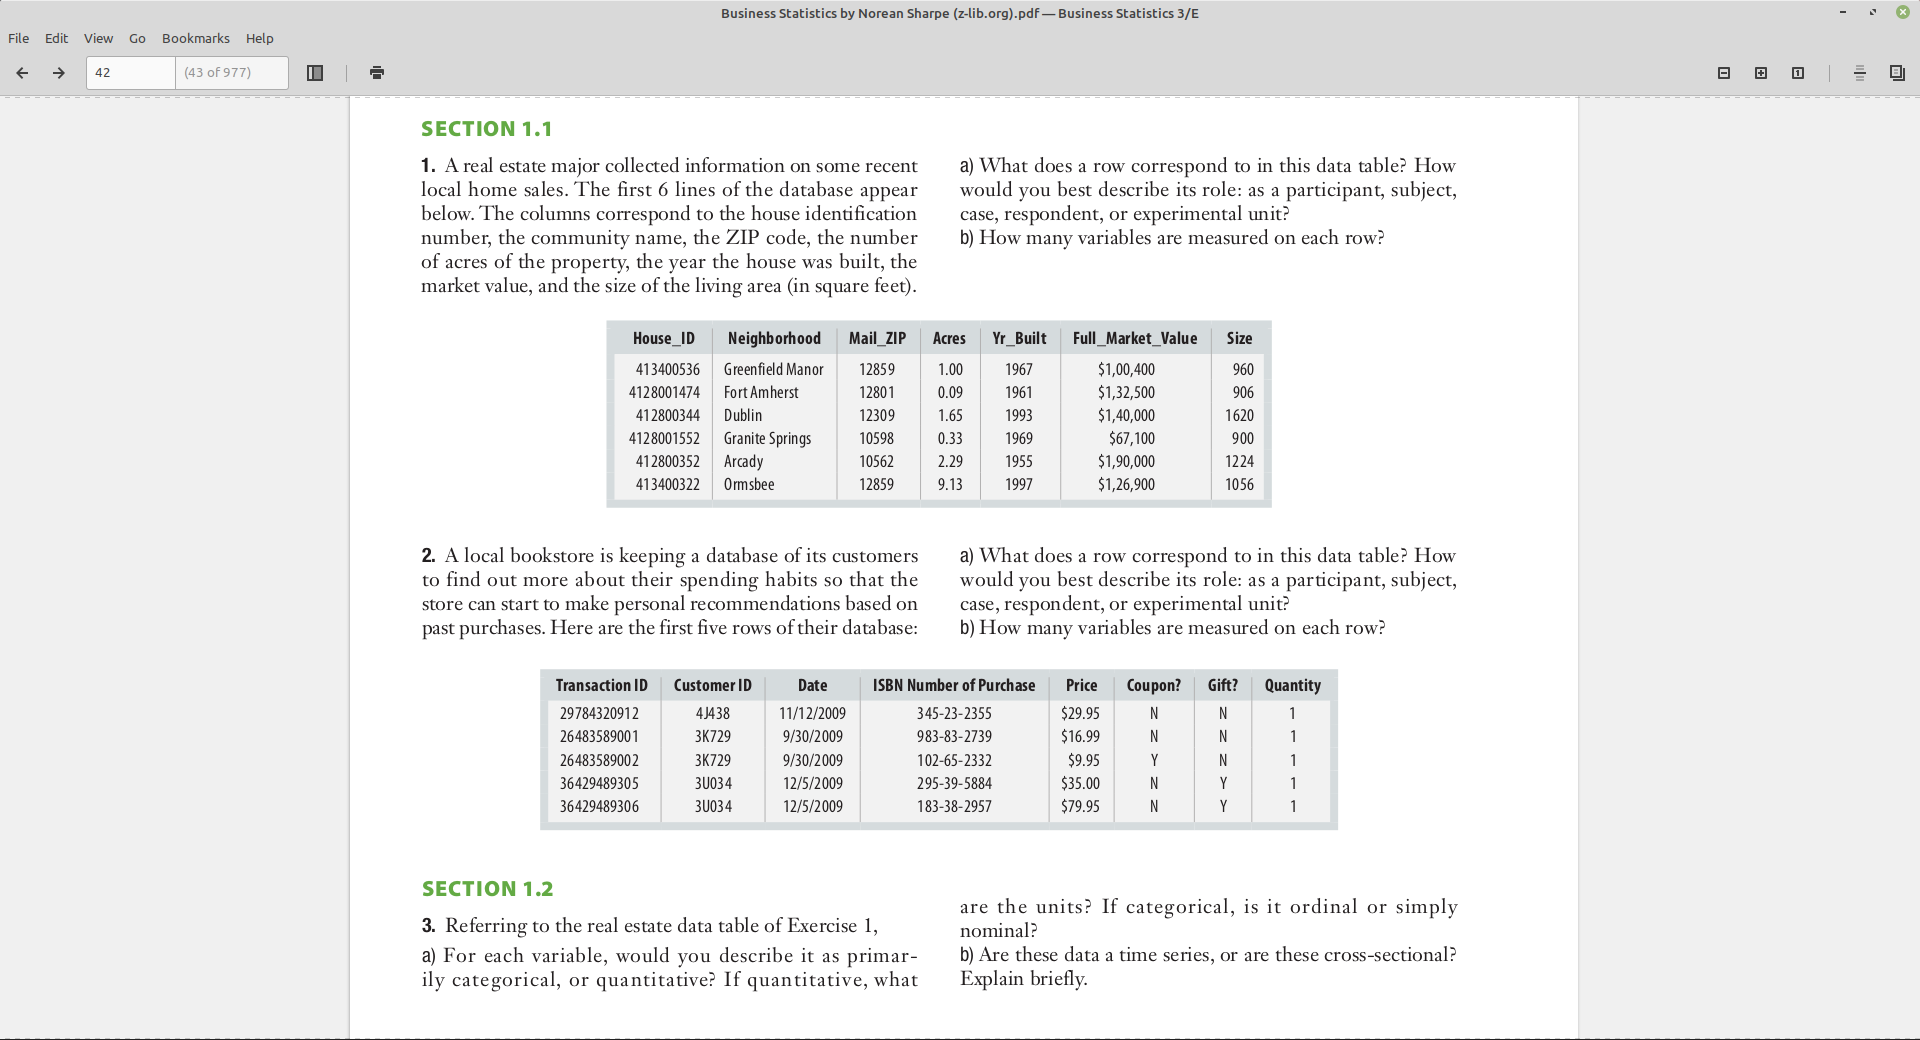
\includegraphics{exercise.png}
\caption{Check out these questions}
\end{figure}
\end{frame}

\begin{frame}{Additional resources}
\protect\hypertarget{additional-resources}{}
\begin{itemize}
\item
  What is panel / longitudinal data
\item
  \url{https://www.youtube.com/watch?v=7_GdwN_iwmw}
\end{itemize}
\end{frame}

\end{document}
